\documentclass[]{article}

\usepackage{graphicx}

%opening
\title{Pareto-heuristic for Flowshop Schedules}
\author{}

\begin{document}
\date{}
\maketitle

\section{Overview}

The flow-shop scheduler created by Umar Waqas et. al. in the context of the Oc\'e paper path scheduling has been investigated in a paper. The ranking method employed in the original scheduler depends on its effectiveness depends on reverse iteration (i.e. last page of job is scheduled first), and on the ranks of individual choices. In this algorithm only one alternative is carried through to the final decision. 

It turns out it is very difficult to predict when (and how) to make the trade-off between aggressively optimizing for productivity, and when to leave room for other kinds of pages in the return path. To enable efficient optimization, it only checks feasibility of schedules when they are considered for selection (i.e. they have the highest rank). This does not improve the worst case complexity, but it does offer a lower average-case complexity.

The ASAP starting times of the operations are checked with the Bellman-Ford algorithm. This algorithm also provides the feasibility check necessary for guaranteeing that the deadlines of operations are obeyed. This algorithm constitutes most of the complexity (and runtime) of the total heuristic, and to achieve high average-case run-times, it is good to call it only when really necessary.

We investigate in the Pareto-heuristic if we can use a set solutions that are trade-offs, with the goal of avoiding purging too many solutions from the search space at once, which should lead to higher-quality schedules, at the cost of higher average execution times. 

\section{Metrics}

The original heuristic contained a ranking method that consisted of a weighted combination of two metrics: the (relative) flexibility and productivity of a choice. As there is only one 'base' schedule on which the choice is applied, this leads to a ranking that is able to estimate which choice might be best to continue with. Such choices are local, and do not (necessarily) describe the resulting schedules. They cannot easily be compared, as the history of the choices may not be reflected in the ranking of the current choice, while it does make a difference.

Even though tuning of the weights has led to reasonable results, the results in certain categories have now been outperformed by the inclusion of pattern detection in the Eager Scheduler. These (for Oc\'e important) categories are the Booklet patterns. These have a predictable structure where a little bit of space needs to be left for the (predictable) cover sheet to be interleaved. It is not possible to make the existing heuristic optimize both for homogeneous sheets (almost maximally greedily adding pages for 'local' high productivity) and with the same settings optimize for Booklet and 'random' type jobs.

\subsection{Desired properties}

It is difficult to say when losing flexibility to gain productivity is beneficial for the overall schedule. Even when taking into account several productivity vs flexibility trade-offs, it is not trivial to see how to define these actions. Especially in the Oc\'e case, you don't want to keep flexibility for eternity, as this will definitely harm the productivity. It is interesting to keep trade-offs that contain: 
\begin{itemize}
\item a very flexible schedule (i.e. larger pages can be interleaved)
\item a 'strictly periodic' schedule (i.e. no more than the currently being printed sheets can be interleaved), which is beneficial for homogeneous schedules
\end{itemize}


\subsubsection{Relative importance of history of metrics}
As we aim to make local approximations of the quality of a schedule, it may occur that past decisions which do not have an impact on further schedulability have a larger influence than the current choices (in flexibility). Then we need to take into account that such impact needs to be diminished over time, for example, take diminishing flexibility of choices:
$F_n = F(c_n) + \alpha F_{n-1}$ 

Especially in the Oc\'e case, the deadlines are remarkably structured; each page needs to come back at a certain point in time, but this deadline exists only between the first and second pass of the page (i.e. the second and third operation of the job in the equivalent flow-shop).

\subsubsection{Efficiency of metrics}
For each scheduling choice we can make, it is best if we can avoid to depend on the (expensive) Bellman Ford algorithm. Any metric that we devise should therefore be independent of the ASAP times (or can work on an 'approximate' ASAP schedule, calculated in the 'base' schedule). This would make the algorithm very fast on average case, while the worst case remains the same.

We aim to compute the metrics in a better worst case complexity than $O(n \log n)$.

\subsubsection{Measuring metric similarity}
As we have a powerful set of metrics to define trade-offs (makespan and sum-of-slacks), which is costly to compute, we can try to 'emulate' these metrics by seeing if their predictive value can be matched with more computationally efficient metrics. We can test these assumptions by checking if there exists a correlation between the metrics. Although a different choice in the start of the algorithm may lead to different schedules and follow-up choices, at least this correlation will yield us some insight into whether it has a high chance of taking the same decisions based on the simpler metrics.

This allows us to dump the metrics calculated in each iteration of the algorithm, and compare the similarity of the metrics, without having to run different experiments.


\subsection{Flexibility}
Flexibility is the capability of a schedule to interleave future pages, based on the scheduling choices made \textit{so far}. The most flexible schedule is one where no pages are interleaved, and the least flexible schedule is one where no pages can be interleaved.

One way to measure this is to see how far each operation is from it's deadline. This can be measured in $O(n)$ time after the ASAP times are calculated (which takes $O(n^3)$).

\subsubsection{Flexibility approximation}


\subsection{Productivity}
Productivity is the measure that defines how effective the (partial schedule) is in processing the jobs scheduled \textit{so far}.

\section{Observations}
When checking if a choice makes a schedule less flexible, or more productive, then we can locally check whether or not the additional time introduced by the outgoing edge of the choice will lead to an increase in the ASAP time of the outgoing edge's destination node. If this is the case, then the productivity will be impacted.

\section{Extra remarks}
Check deadlines in $O(d)$? where $d = n$, or $d = n^3$. 

Possible to have a list with 'holes' between operations? (or something equivalent), so that you can stop at a certain point, if you know that they won't be able to be interleaved any more? I.e. discard choices as soon as possible.

\begin{figure}
\centering
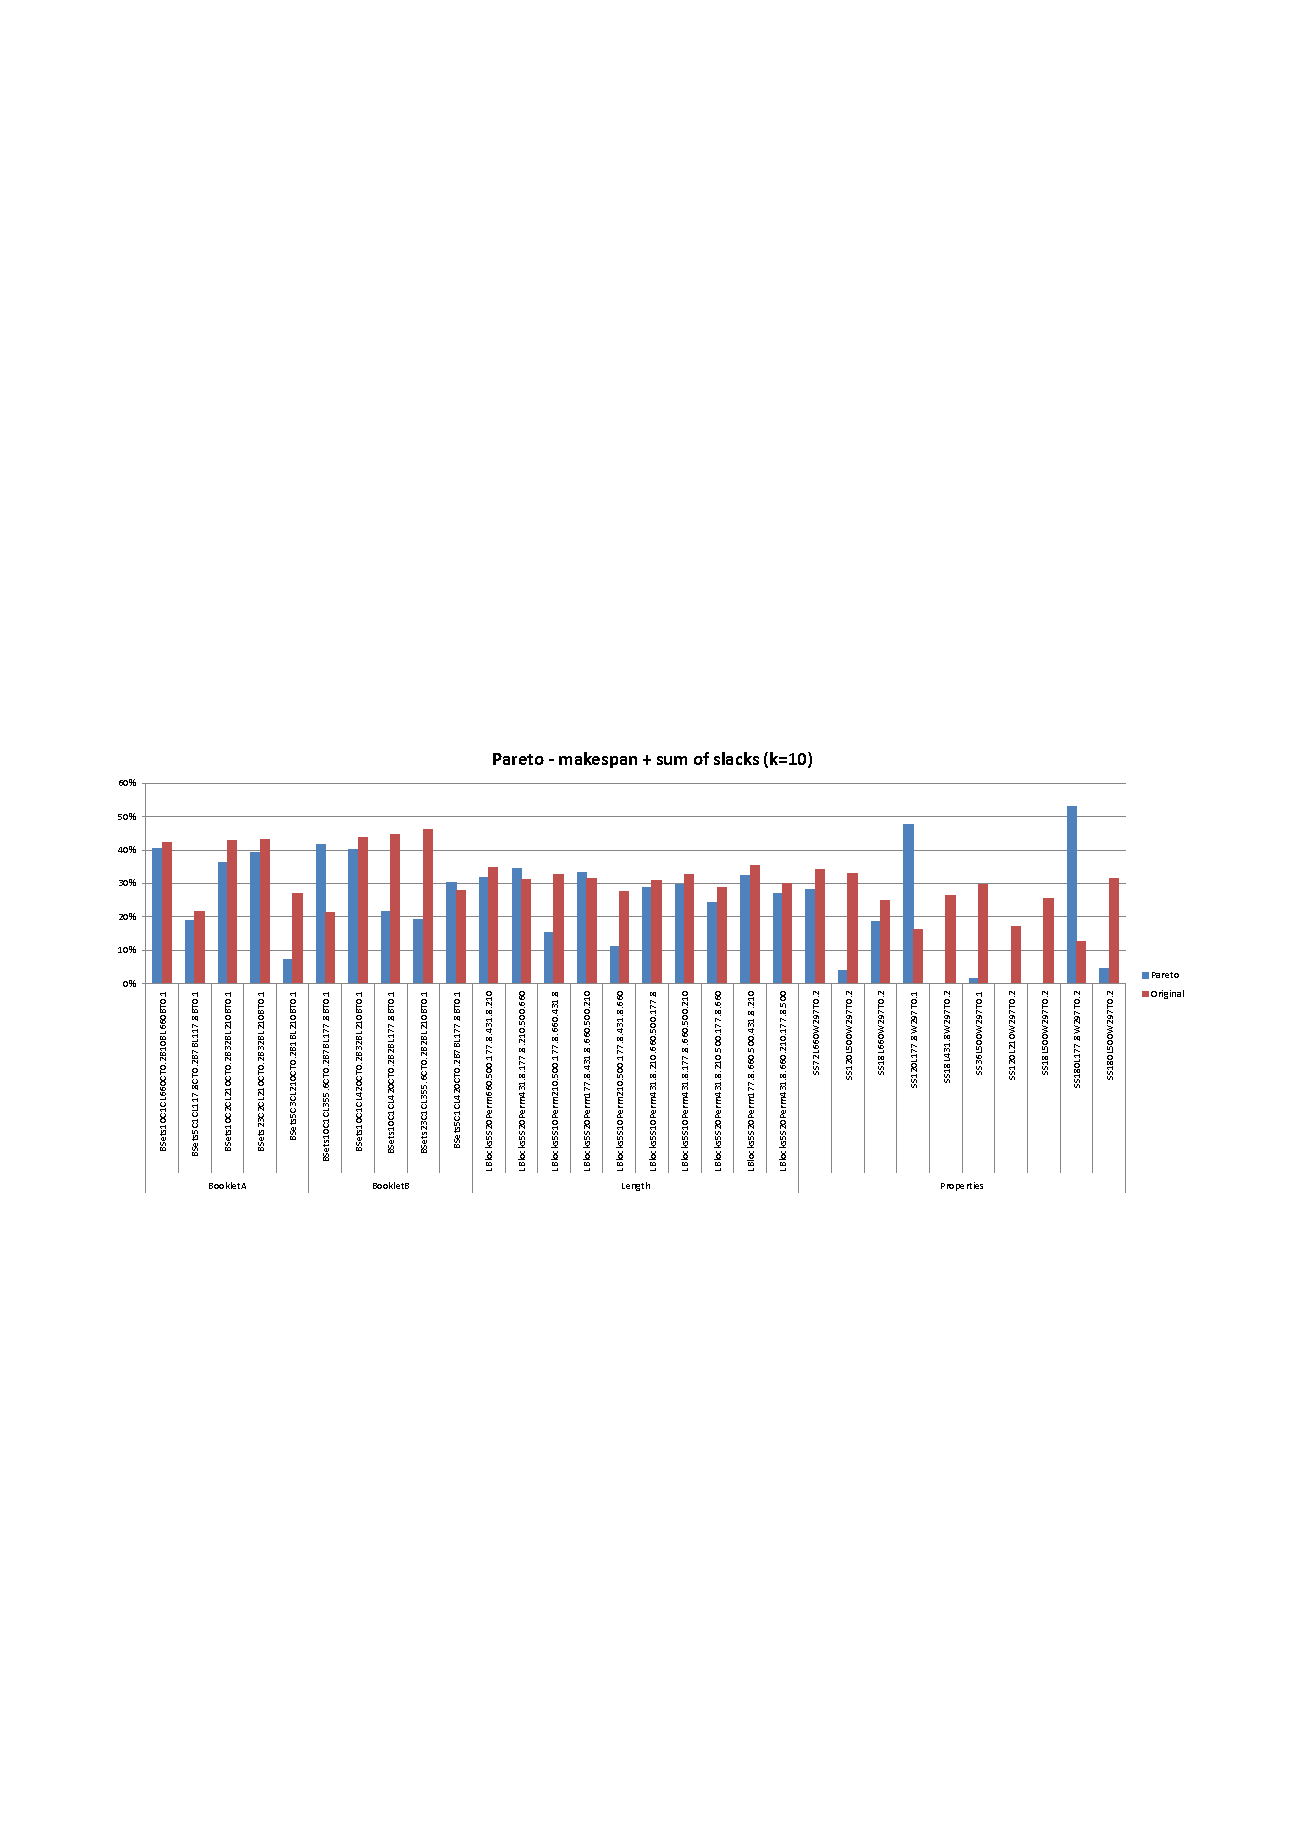
\includegraphics[width=\textwidth]{subset-benchmark-makespan.pdf}
\caption{Makespan comparison for Pareto with makespan and sum-of-slacks metrics (k=10)}
\label{fig:subset-benchmark-makespan}
\end{figure}
\begin{figure}
\centering
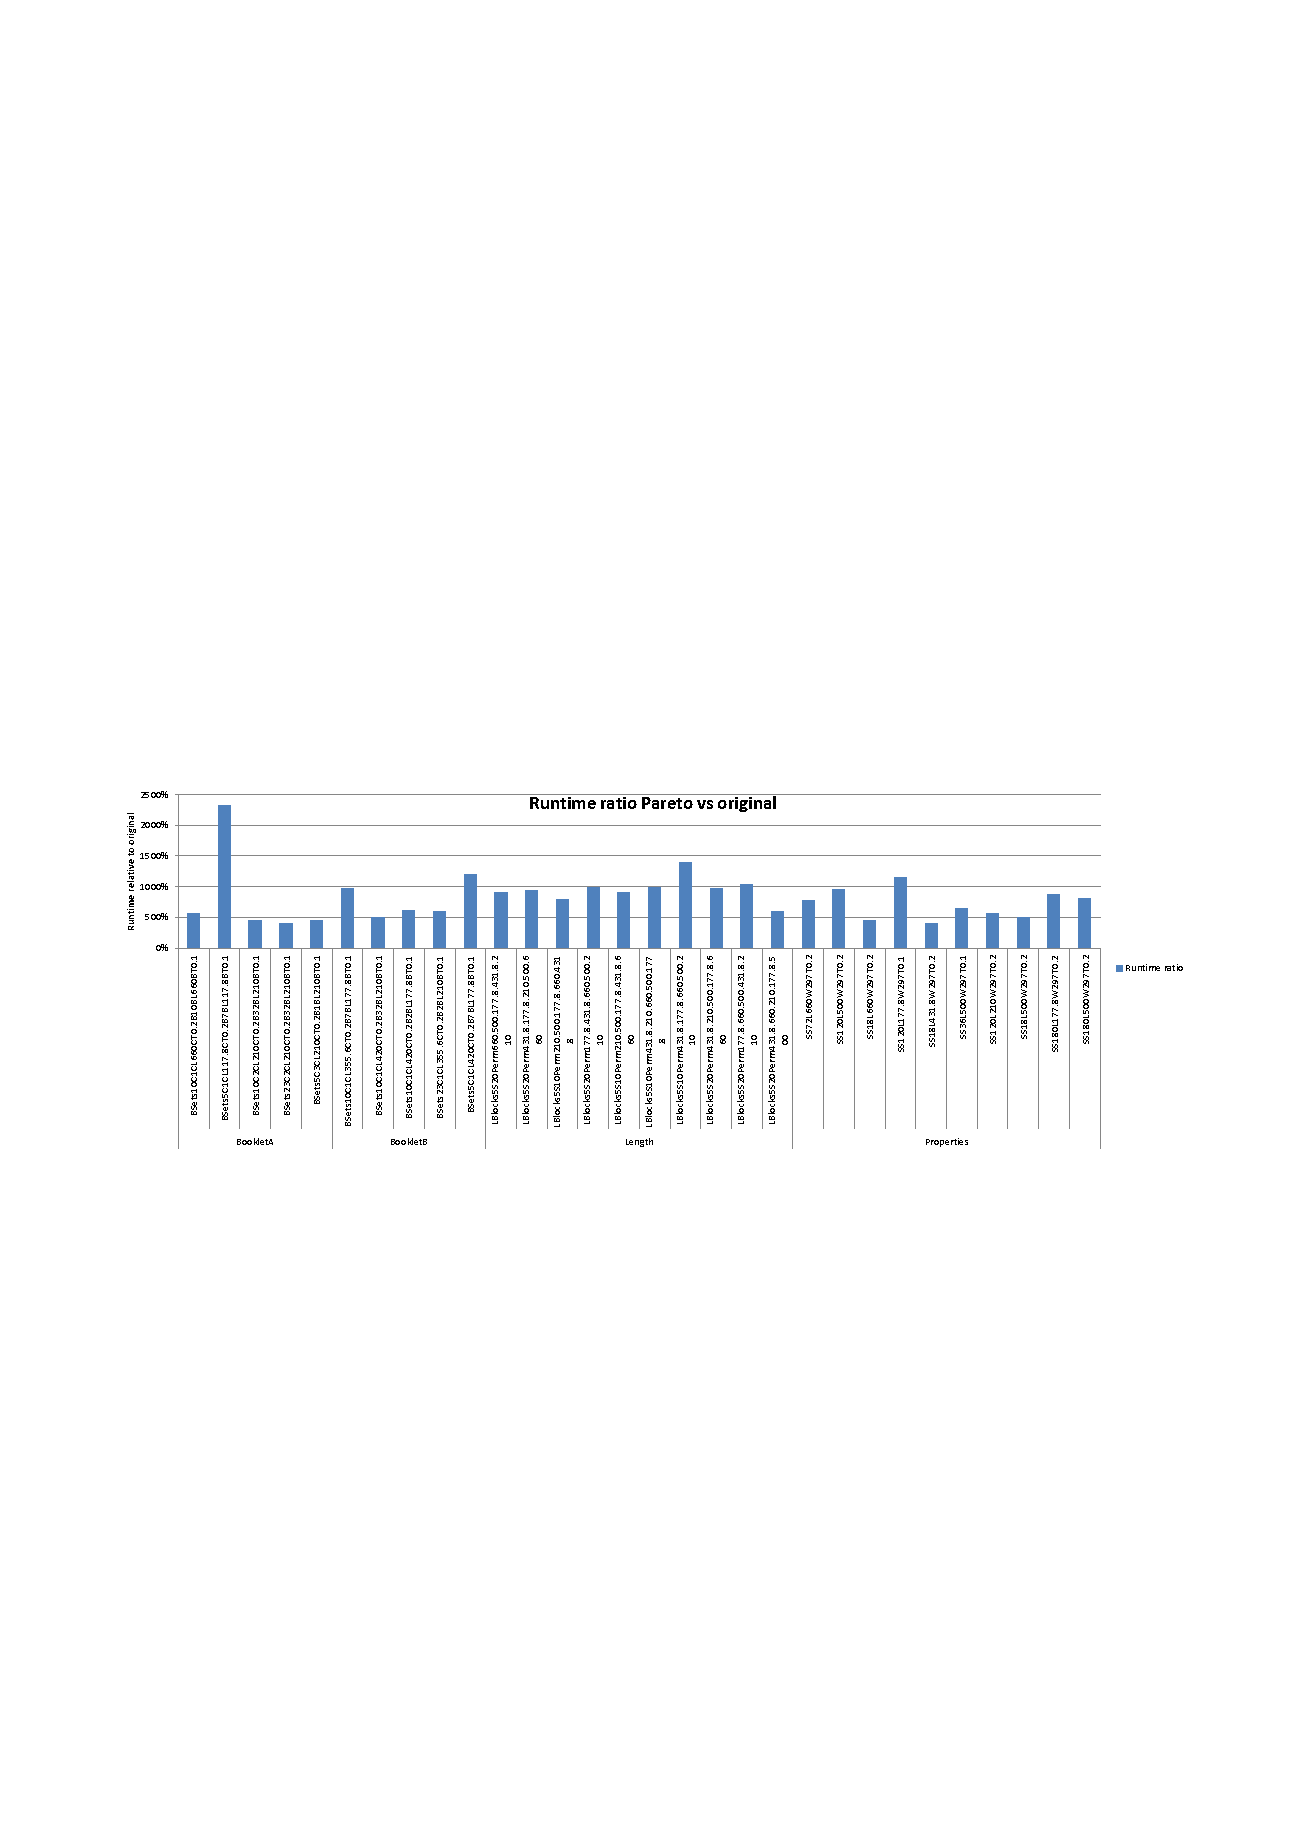
\includegraphics[width=\linewidth]{subset-benchmark-runtime.pdf}
\caption{Runtime comparison for Pareto with makespan and sum-of-slacks metrics (k=10)}
\label{fig:subset-benchmark-runtime}
\end{figure}


\end{document}
